\documentclass[11pt]{article}
\pdfoutput=1
\usepackage{simplemargins}
\usepackage{url}
\usepackage[pdftex]{graphicx}
\usepackage{setspace}
\graphicspath{{figures/}}
\usepackage{siunitx}
\setlength{\parindent}{0pt} 
\setlength{\parskip}{1.6ex} 
\setallmargins{1in} 
\linespread{1.6}
\usepackage[round]{natbib}
\listfiles

\begin{document}

% Title must be 150 characters or less
\begin{flushleft} 
\singlespacing
{\Large \textbf{The genetic architecture of local adaptation I: The genomic landscape of 
foxtail pine (\textit{Pinus balfouriana} Grev. \& Balf.)}}
% Insert Author names, affiliations and corresponding author email.
\null

Christopher J.\ Friedline$^{1}$, 
Brandon M. Lind$^{1}$,
Erin M. Hobson,$^{1}$,
Douglas E. Harwood$^{1}$, 
Annette Delfino Mix$^{2}$,
Patricia E. Maloney$^{3}$, and
Andrew J. Eckert$^{1,4}$
\null

\bf{1} Department of Biology, Virginia Commonwealth University, Richmond, VA 23225
\\
\bf{2} Institute of Forest Genetics, USDA Pacific Southwest Research Station, Placerville, 
CA 95667
\\
\bf{3} Department of Plant Pathology, University of California, Davis, CA 95616
\\
\bf{4} Author for Correspondence
\null

$\ast$ E-mail: aeckert2@vcu.edu
\end{flushleft}

\section*{Abstract}

\section*{Introduction}
The genetic architecture of fitness-related traits has been a major focus of geneticists for 
over a century. Genetic architecture refers to the number, type, effect size, genomic organization, 
interactions, and environmental dependency of the loci contributing to phenotypic variation 
which in turn creates variation in fitness among individuals within populations \citep{Eckert:2012a}. 
Interest in this architecture stems from the want to explain the nature of genetic variation which 
contributes to evolution via the accumulation of adaptations within lineages (i.e. adaptive evolution).
Evidence for adaptive evolution among populations of plants is commonly documented at both the phenotypic 
and molecular genetic levels \citep{Kawecki:2004, Pannell:2013}, so that some of the best
examples of adaptive evolution within lineages comes from the field of plant genetics.
Early efforts to understand the genetic architecture of fitness-related traits
focused primarily on the number and effect size of the loci underlying heritable, phenotypic variation \citep{Fisher:1930}. 
Recent work has extended this line of research, with myriad studies linking phenotypic with genetic variation 
through linkage mapping, both within pedigrees \citep{Mauricio:2001, Neale:2011, Ritland:2011} and within 
unstructured populations \citep{Ingvarsson:2011, Eckert:2013a}, 
or through quantitative genetic experimentation \citep{Anderson:2013a, Anderson:2013b, Fournier-Level:2013}. All of these approaches 
have been used extensively in forest genetics, with local adaptation among forest tree populations clearly
being documented over the past century \citep{White:2007, Neale:2011}. Despite great advances in experimental technology, empirical 
focus has remained almost fully on the number, effect size, type, and interactions among loci contributing 
to adaptive evolution \citep{Neale:2011, Alberto:2013}. The genomic organization of such loci, however, 
is also relevant, as it affects many of the other attributes of genetic architecture listed previously 
\citep{Kirkpatrick:2006, Yeaman:2011, Yeaman:2013}, including the ability to detect the loci as underlying trait variation. 
Any thorough examination of the genetic architecture of fitness-related traits, therefore, should include 
some aspect of the genomic organization of the loci contributing to trait variation. Here, we leverage 
this idea in the first of a series of papers dissecting the genetic architecture of fitness-related 
traits in a non-model conifer species, foxtail pine (\textit{Pinus balfouriana} Grev. \& Balf.), with the 
ultimate goal of testing explicit evolutionary hypotheses about the genomic organization of loci 
contributing to variation in fitness-related traits.

Ideally, the genomic organization of loci contributing to variation in fitness-related traits would follow 
naturally from the production of a genome sequence (i.e. a physical map). For many taxa, especially those with 
small to modest genome sizes, this is monetarily and computationally feasible using next-generation DNA sequencing 
technologies \citep{Koboldt:2013}. For taxa with large or complex genomes, however, even the advent of next generation DNA 
sequencing does not solve the complexity and cost hurdles associated with the production of a finished genome sequence. Conifers have large and 
complex genomes \citep{Murray:1998, Ahuja:2005}, with estimated average genome sizes in \textit{Pinus} in the 
range of \SIrange{20}{30}{Gbp}. Several genome projects, each involving many laboratories, are underway or have been 
completed \citep{Mackay:2012}. Even these efforts often initially result in limited information, 
as current assemblies of the Norway spruce (\textit{Picea abies} L.) and loblolly pine (\textit{Pinus taeda} L.) genomes 
contain millions of unordered contigs with average sizes in the thousands of base pairs \citep{Nystedt:2013}. An alternative, but not mutually exclusive, approach to describing the genome of an organism 
is that of linkage mapping. In this approach, genetic markers are ordered through observations of recombination events 
within pedigrees. This approach dates to the beginning of genetics and the logic has remained relatively unchanged 
since the first linkage maps were created in \textit{Drosophila} \citep{Sturtevant:1913}.

Renewed interest in linkage maps has occurred for two basic reasons. First, linkage maps can be used to order contigs 
created during genome sequencing projects \citep{Mackay:2012, Martinez-Garcia:2013}. In this fashion, linkage 
maps are used to help create larger contigs from those generated during the assembly. It is these larger contigs that 
create the utility that most practicing scientists attribute to genome sequences. Second, linkage maps are relatively 
easy to produce and provide a rich context with which to interpret population and quantitative genetic patterns of variation 
\citep[e.g.][]{Eckert:2010a, Eckert:2010b, Eckert:2013a, Yeaman:2013}. They can also be used to test explicit hypotheses about 
the organization of loci contributing to adaptive evolution. For example, \citet{Yeaman:2011} developed theoretical 
predictions about the genomic organization of loci underlying patterns of local adaptation as a function of gene flow, 
so that loci contributing to local adaptation have differing spatial structure within genomes as a result of differing 
regimes of gene flow. The relevant scale \citep[\textit{sensu}][]{Houle:2011} in these mathematical formulations is that 
of recombinational distance among loci, as it is recombination that breaks apart advantageous allelic combinations across 
loci, so that when matched with an appropriate study system, linkage maps provide the impetus to test basic evolutionary 
hypotheses. In this context, future additions of finished genome sequences will add only to the interpretation of 
results based on linkage maps.

Construction of linkage maps have a long history within forest genetics, mostly through their use in quantitative trait locus mapping \citep{Ritland:2011}. 
Conifers in particular are highly amenable to linkage mapping, with approximately 25 different species currently having some 
form of linkage map \citep[see Table 5-1 in][]{Ritland:2011}. Much of the amenability of conifers to linkage mapping stems from 
the early establishment of breeding populations in economically important species and from the presence of a multicellular 
female gametophyte (i.e. the megagametophyte) from which the haploid product of maternal meiosis can be observed \citep{Cairney:2007}. Indeed, many of the first linkage maps in conifers were generated from collections of 
megagametophytes made from single trees \citep{Tulsieram:1992, Nelson:1993, Kubisiak:1996}. Continued development 
of genetic marker technologies has facilitated rapid development of linkage maps across a diversity of species, with the largest maps 
generated for economically important species \citep[e.g.][] {Achere:2004, Kang:2010, Martinez-Garcia:2013}. 
The development of biologically informative markers in non-economically important conifers, however, was hampered by production cost of markers. 
For example, the vast majority of linkage maps outside of economically important species were created with uncharacterized genetic 
markers \citep[e.g.][]{Travis:1998}. The majority of this cost previously was in the two-step approach needed to generate biologically 
meaningful markers: polymorphism discovery via DNA sequencing of genic regions followed by genotyping of polymorphisms 
discovered in step one \citep[cf.][]{Eckert:2013a}. As such, much of the knowledge about the genetic architecture of fitness-related 
traits outside of a handful of economically important conifer species was about the number and effect size of uncharacterized 
genetic markers \citep{Ritland:2011}. Cost restrictions, however, have largely disappeared 
as it is now feasible to jointly discover polymorphisms and genotype samples using high-throughput DNA sequencing approaches such as restriction-associated 
DNA sequencing \citep [RADseq; e.g.][] {Peterson:2012}. 

The generation of dense linkage maps from RADseq data is a complex endeavor due to the inherent stochasticity
and error prone nature of the generation and analysis of short read data. Recent examples in several crop species highlight the
difficulties that must be overcome with respect to missing data and errors in calling polymorphic sites and the resulting genotypes\citep{Pfender:2011, Ward:2013}. RADseq has been 
successively applied to samples taken from natural populations of non-model conifer species \citep{Parchman:2012}, but has not yet 
been applied to linkage mapping in these species, so that an exploration of these methods to linkage mapping in the large and complex 
genomes of conifers is warranted. Here, we take this approach using megagametophyte arrays from four maternal trees of foxtail pine
to generate maternal linkage maps comprised of tens of thousands of markers. There are currently no published linkage 
maps for this species nor any within the subsection \textit{Balfourianae}. By doing so, we examine the inherent biases
to RADseq data generation in conifer genomes and how these biases affect downstream inferences of linkage maps. We subsequently discuss
the utility of our inferred linkage maps to comparative genomics within the conifers and to future tests of how patterns of gene flow 
affect the genomic organization of loci underlying fitness-related traits.


\section*{Materials and Methods}

\subsection*{Focal species}
Foxtail pine is a five needle species of \textit{Pinus} classified into 
subsection \textit{Balfourianae}, section \textit{Parrya}, and subgenus \textit{Strobus} 
\citep{Gernandt:2005}. It is one of three species within subsection \textit{Balfourianae} 
\citep{Bailey:1970} and generally is regarded as the sister species to Great Basin bristlecone pine \citep[\textit{P. longaeva}; see][] 
{Eckert:2006a}. The natural range of foxtail pine encompasses two 
regional populations located within California that are separated by approximately 500 km - 
the Klamath Mountains of northern California and the Sierra Nevada of southern California 
(Figure 1). These regional populations diverged approximately one million years ago (mya), 
with current levels of gene flow between regional populations being approximately zero 
\citep{Eckert:2008}. Within each regional population, levels of genetic diversity and the 
degree of differentiation among local stands differ, with genetic diversity being highest in 
the southern Sierra Nevada population and genetic differentiation being the highest in the 
Klamath population \citep{Oline:2000, Eckert:2006b, Eckert:2008}. These two regional populations
have also been recognized as distinct subspecies based on numerous quantitative traits, with \textit{P. balfouriana}
subsp. \textit{balfouriana} located in the Klamath region and \textit{P. balfouriana} subsp. \textit{austrina} located in the southern
Sierra Nevada mountains \citep{Mastrogiuseppe:1980}. The two regional populations of foxtail pine 
thus represent a powerful natural experiment within which to examine the genomic organization of loci contributing to local adaptation. 

\subsection*{Sampling}
Seed lots from 141 maternal trees distributed throughout the natural range 
of foxtail pine were obtained during 2011 and 2012. Of these 141 maternal trees, 72 were sampled from the 
Klamath region, while 69 were sampled from the southern Sierra Nevada region. These 141 families were
divided among 15 local stands ($n = 4$ to $17$ trees/stand), with eight stands in the Klamath region and seven stands in the southern Sierra Nevada.
Approximately 50 seeds were germinated from each seed lot and 35 of those 50 seedlings were planted in a 
common garden located at the USDA Institute of Forest Genetics, Placerville, California. The 
common garden was established using a randomized block design and involved three separate plantings of seeds spanning
approximately one year from June 6, 2012 until May 20, 2013. Four of the 141 maternal trees were selected 
at random ($n = 2$ from the Klamath region and $n = 2$ from the southern Sierra Nevada) for linkage analysis. 
For each of these trees, \SIrange{75}{100}{} seeds were germinated and planted in the common garden. 
Upon germination, haploid megagametophyte tissue was rescued from each seedling, cleaned, and stored for further 
analysis in \SI{1.5}{\mL} Eppendorf tubes at \SI{-20}{\celsius}.


\subsection*{Library Preparation and Sequencing}
Total genomic DNA was isolated from each rescued megagametophyte using the DNeasy 96 Plant 
kit following the manufacturer’s protocol (Qiagen, Germantown, MD). RADseq \citep{Davey:2010, Parchman:2012, Peterson:2012} 
was used to generate a genome-wide set of 
single nucleotide polymorphism (SNP) markers for linkage mapping following the protocol 
outlined by \citet{Parchman:2012}. In brief, this protocol is a double digestion RADseq 
approach based on digestion of total genomic DNA using EcoRI and MseI followed by single-end 
sequencing on the Illumina HiSeq platform. Following digestion, adaptors 
containing amplification and sequencing primers, as well as barcodes for multiplexing, 
were ligated on to digested DNA fragments. We chose to multiplex 96 samples using the 
barcodes available from \citet{Parchman:2012}. These barcodes are a mixture of eight, nine, and 
10 bp tags that differ by at least four bases, so as to accommodate sample identification in the 
presence of sequencing errors. Following ligation, successfully ligated DNA fragments were 
amplified using PCR and amplified fragments were size selected using gel electrophoresis. We selected 
fragments in the size range of 400 bp (\SIrange{300}{500}{bp}) by excising and purifying pooled DNA from 2.5\% 
agarose gels using QIAquick Gel Extraction Kits (Qiagen). Further details, including relevant reagents and 
oligonucleotide sequences, can be found in File S1. All DNA sequencing was performed on the Illumina HiSeq 2000 or 2500
platform at the VCU Nucleic Acids Research Facility (\url{http://www.narf.vcu.edu/}).


\subsection*{DNA Sequence Analysis}

There are multiple steps involved with the processing of raw DNA sequence reads into a set of SNP genotypes that are useful for linkage mapping:
(1) quality control, filtering, and demultiplexing, (2) assembly to generate a reference sequence for mapping reads, (3) mapping 
of reads to call SNPs and genotypes for each sample, and (4) filtering of SNPs and the resulting genotypes for
data quality and biological meaning.

DNA sequence reads were demultiplexed into sample-level fastq files, following quality control 
and filtering.  The filtering pipeline was adapted from \citep{Friedline:2012fm}, and is briefly: reads 
containing any N beyond the first base were excluded. Reads having N as the first base were shifted 
to exclude it.  Additional quality filtering ensured that all reads in the resulting set for downstream 
processing had a minimum average quality score of 30 over 5 base-pair (bp), overlapping windows 
and that not more than \SI{20}{\percent} of the bases had quality scores below 30. Reads passing the 
quality control steps were demultiplexed into sample-specific fastq files by exact pattern matching to 
known barcodes.

From each set of demultiplexed reads, the individual with the largest number of reads as assembled using 
Velvet (Zerbino, version 1.2.10), with hash length ($k$) coverage cutoff optimized using parameter sweeps of $k$ 
through the contributed VelvetOptimiser (\url{http://www.vicbioinformatics.com}, version 2.2.5) 
script (for odd $k$ on $k=[19,65]$).  Assembly robustness was evaluated in each case using the LAP likelihood 
framework \citep{Ghodsi:2013bc}, version 1.1, averaged across five iterations to account for variance 
in the likelihood calcuations.  Each assembly was also indexed and aligned (Figure \ref{f:mapping_performance}) 
to the original set of reads 
using Bowtie2 \citep{Langmead:2012jh} (\texttt{--local --very-sensitive}) and compared the average maximum 
likelihood estimate. In all cases, the assembly with the highest average maximum likelihood value was 
chosen as the reference for SNP calling.

SNPs were called for all individuals against their respective reference using a medley of methods.  First, 
reads were mapped to the reference with Bowtie2 (\texttt{--local --very-sensitive-local}).  These resulting 
sam files were converted their binary equivalent (e.g., bam) using \texttt{samtools} version 0.1.19 
(\texttt{view, sort, index}) \citep{Li:2009ka}.  SNPs were called using \texttt{bcftools} and filtered using 
\texttt{vcfutils} to exclude SNPs with less than 100x coverage. The resulting variant call files (vcf) 
were further processed using \texttt{vcftools} version 0.1.11 (cite) to remove indels and exclude genotype 
calls below a quality threshold of 5, and output as a matrix (\texttt{--012}) of genotypes by individuals.  
To ensure that only SNPs that sort according to expected ratios, we excluded SNPs using a $\chi^2$ test of 
homogeneity against an expectation of 1:1 segregation. This segregation pattern was expected, because
the maternal tree had to be a heterozygote for us to detect a SNP and Mendel's first law guarantees
that 

\subsection*{Linkage Analysis}

The production of a genetic linkage map for a single tree requires three main steps: (1) calculation of 
pairwise distances between all pairs of loci, (2) clustering of loci based on these pairwise distances, 
and (3) ordering of loci within each cluster.  A variety of software packages exist to carry out these steps (XXXXX).
Traditional software packages for linkage mapping, however, are not amenable to large amounts of missing data and frequent
errors in genotype calls. The former causes issues with all aspects of analysis, while the latter primarily affects the 
genetic distances between markers (XXXXX). We thus followed the approach of \citet{Ward:2013}, which was designed specifically for RADseq
data. Pairwise distances were estimated and loci were clustered using a custom R script (see File S2). We used MSTmap \citep{Wu:2008} 
to infer marker order and Maskov \citep{Ward:2013} to impute and correct genotypes. These two programs
were used iteratively. MSTmap was used initially to order markers, which was followed by the use of Maskov
to impute and correct putative genotype errors conditional on this initial marker ordering. A last round of ordering 
was performed using MSTmap conditional on the imputed and error corrected genotype data. 

The relevant pairwise distance for genetic linkage mapping is the standardized number of recombination events separating
the haplotypes of two related individuals.  As defined, this distance can be calculated for a set of biallelic loci using the Hamming distance.
The Hamming distance is the number of differences separating two binary strings. Here, the binary strings are the haploid
genotypes for the set of two megagametophytes. This distance was shown to have as its expected value the number of recombination
events separating two haplotypes (XXXX).



\subsection*{Sensitivity Analysis}

\section*{Results}

\section*{Discussion}

\section*{Acknowledgements}

The authors would like to thank the staff at the USDA Institute of Forest Genetics, the 
VCU Nucleic Acids Research Facility, and the VCU Center for High Performance Computing. 
In addition, we would like to thank Tom Blush and Tom Burt for help in obtaining 
seeds. Funding for this project was made available to AJE via start-up funds from Virginia 
Commonwealth University. CJF was supported by the National Science Foundation (NSF) National Plant Genome 
Initiative (NPGI): Postdoctoral Research Fellowship in Biology (PRFB) FY 2013 Award \#NSF-NPGI-PRFB-1306622.

\clearpage

\singlespacing
\bibliographystyle{spbasic}
\bibliography{refs}

\clearpage

\begin{figure}[t]
\centering
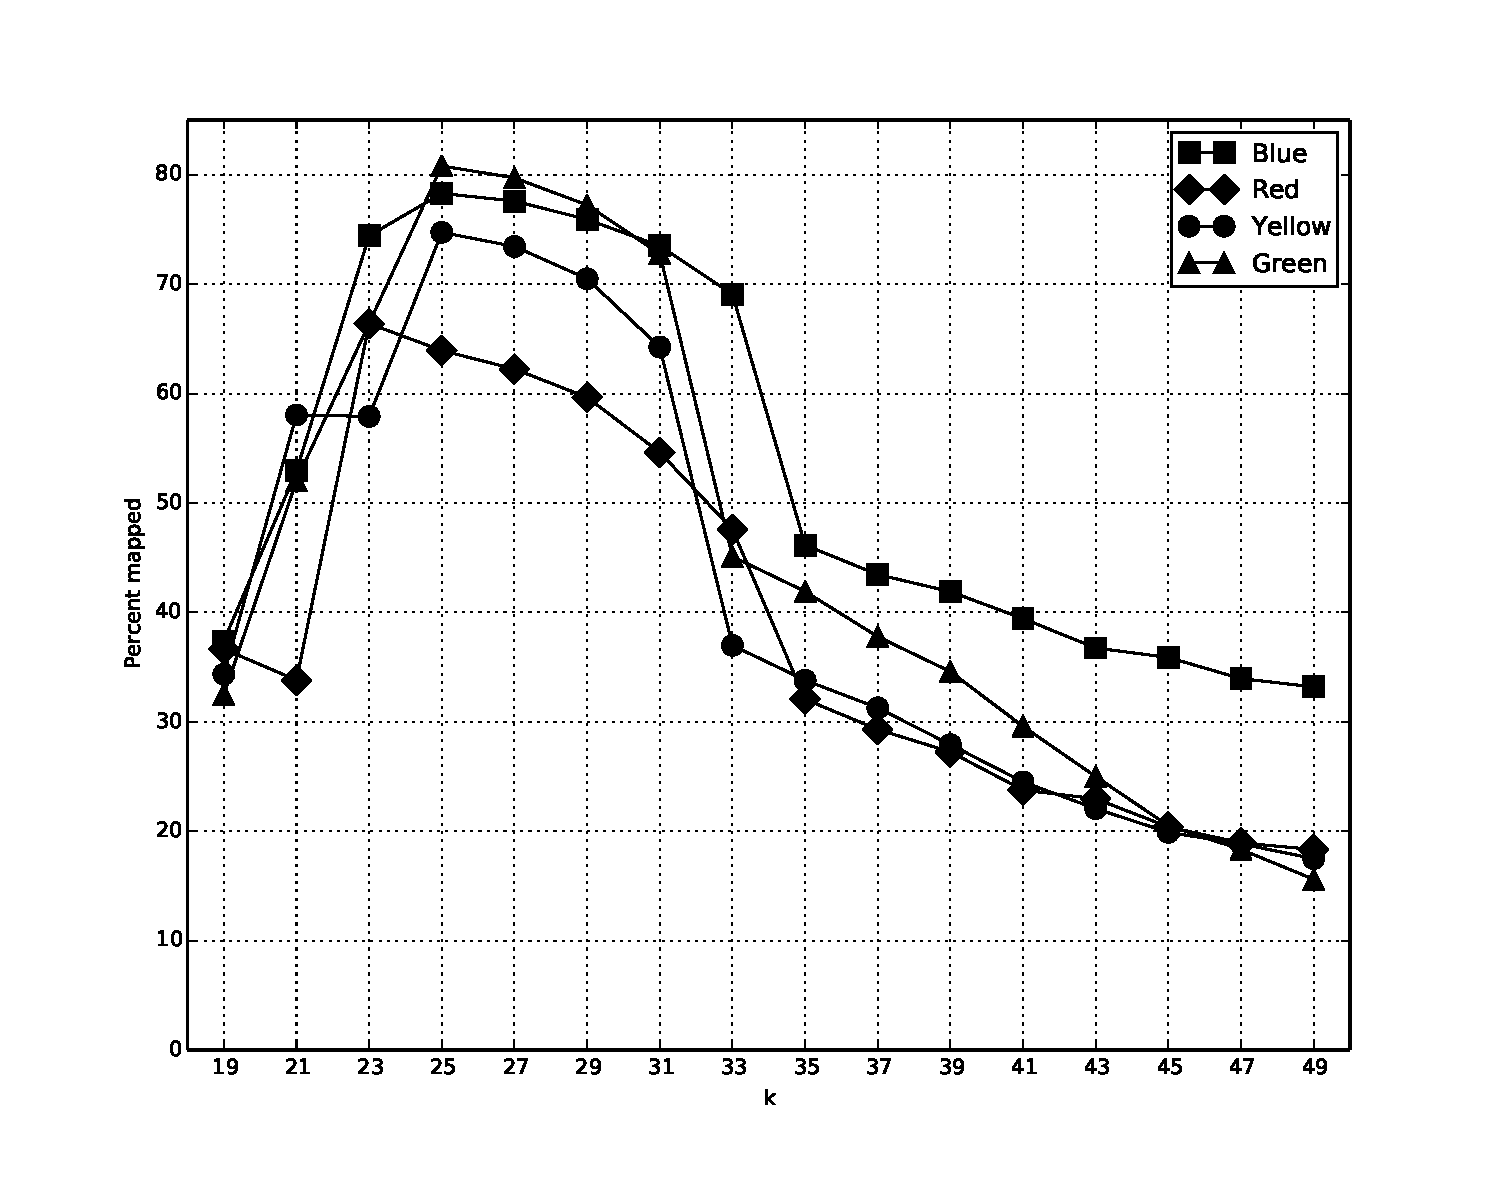
\includegraphics[width=1.0\textwidth]{mapping_performance}
\caption{Mapping performance at various sizes of $k$ for all four assemblies.  Assemblies using 
$k>53$ were excluded from the figure.}
\label{f:mapping_performance}
\end{figure}

\end{document}
